\documentclass[11pt, oneside]{article}   	% use "amsart" instead of "article" for AMSLaTeX format


% \usepackage{draftwatermark}
% \SetWatermarkText{Draft}
 % \SetWatermarkScale{5}
% \SetWatermarkLightness {0.85} 
% \SetWatermarkColor[rgb]{0.7,0,0}


\usepackage{geometry}                		% See geometry.pdf to learn the layout options. There are lots.
\geometry{letterpaper}                   		% ... or a4paper or a5paper or ... 
%\geometry{landscape}                		% Activate for for rotated page geometry
%\usepackage[parfill]{parskip}    		% Activate to begin paragraphs with an empty line rather than an indent
\usepackage{graphicx}				% Use pdf, png, jpg, or eps� with pdflatex; use eps in DVI mode
								% TeX will automatically convert eps --> pdf in pdflatex		
\usepackage{amssymb}
\usepackage{mathrsfs}
\usepackage{hyperref}
\usepackage{url}
\usepackage{authblk}
\usepackage{amsmath}
\usepackage{graphicx}
\usepackage{fixltx2e}
\usepackage{hyperref}
\usepackage{alltt}
\usepackage{color}
\usepackage{bigints}

\newcommand{\argmax}{\operatornamewithlimits{argmax}}
\newcommand{\argmin}{\operatornamewithlimits{argmin}}

\title{Notes on Variational Autoencoders}
\author{David Meyer \\ dmm@\{1-4-5.net,uoregon.edu,...\}}
\date{17 Jan 2015}


\begin{document}
\maketitle

\section{Introduction}
\noindent
Variational Autoecoders (VAEs) \cite{Kingma:2013aa} are generative models in which we have examples $X$ that are distributed according to some unknown distribution $P_{gen}(X)$, and our goal is to learn a model $P$ which we can sample from, such that $P$ is as similar as possible to $P_{gen}$. This is a long standing problem in machine learning, where most approaches have had three significant drawbacks. First, they might require strong assumptions about the structure in the data. Second, they might make severe approximations, leading to suboptimal models.  Third, they might rely on computationally expensive inference procedures like Markov Chain Monte Carlo (MCMC). Recent progress in training neural networks as powerful function approximators through backpropagation have provided new ways to think about the problem. VAEs are one such method.


\section{Review: Latent Variable Models}
\noindent
Most of what we'll review in this section is based on two simple but fundamental rules of probability:

\begin{flalign}
\label{eqn:sum_rule}
\text{Sum Rule:}  & \qquad p(\mathcal{X}) = \sum\limits_{y}{}p(\mathcal{X} \cap \mathcal{Y})\\
\label{eqn:product_rule}
\text{Product Rule:} & \qquad p(\mathcal{X},\mathcal{Y}) = p(\mathcal{X}|\mathcal{Y}) p(\mathcal{Y})
\end{flalign}

Note that
\begin{flalign}
p(\Theta, \mathcal{X})  &= p(\mathcal{X},\Theta) \\
p(\Theta, \mathcal{X})  &= p(\Theta|\mathcal{X}) p(\mathcal{X}) \\
p(\mathcal{X}, \Theta)  &= p(\mathcal{X} | \Theta) p(\Theta) \\
p(\Theta | \mathcal{X}) p(\mathcal{X}) &= p(\mathcal{X}|\Theta) p(\Theta)
\end{flalign}

\bigskip
\noindent
Solving for $p(\Theta | \mathcal{X})$ we get Bayes' Theorem

\begin{flalign}
p(\Theta | \mathcal{X}) &= \frac{p(\mathcal{X}|\Theta) p(\Theta)}{p(\mathcal{X})}
\label{eqn:bayes}
\end{flalign}

\bigskip
\noindent
You might also see Bayes' Theorem written using the \emph{Law of Total Probability}\footnote{The Law of Total Probability is a combination of the Sum and Product Rules} which is sometimes written as follows:

\begin{flalign}
p(A) &= \sum\limits_{n}{} p(A \cap B_{n}) \qquad \qquad  \mathbin{\#} \text{by the \emph{Sum Rule} (Equation \ref{eqn:sum_rule})}\\
&= \sum\limits_{n}{} p(A , B_{n})  \qquad \qquad  \;  \; \, \mathbin{\#} \text{in the notation used in Equation \ref{eqn:sum_rule}}\\
&= \sum\limits_{n}{} p(A|B_{n}) p(B_{n})  \qquad \mathbin{\#} \text{by the \emph{Product Rule} (Equation \ref{eqn:product_rule})}
\end{flalign}

\noindent
\subsection{Latent Variables?}
The basic idea here is that the distribution of the data we observe, $\mathcal{X}$,  is controlled (or at least significantly influenced) by a set of hidden or \emph{latent} variables $\mathcal{Z}$.  In many cases what we want to learn is a mapping from the latent variables $z$ to some complicated distribution on $x$.

\bigskip
\noindent
Stated more formally,  for $x \in \mathcal{X}$ and $z \in \mathcal{Z}$ ($z$ is a vector of latent variables, generally with values taken from $\mathbb{R}$):

\begin{flalign}
p(\mathbf{x}) &= \int_{z} p(\mathbf{x},\mathbf{z}) dz\\
        &= \int_{z} p(\mathbf{x}|\mathbf{z}) p(\mathbf{z}) dz \qquad \qquad  \;  \; \, \mathbin{\#} \text{sum and product rules}
\label{eqn:model}        
\end{flalign}

\noindent where $p(\mathbf{z})$ is something simple like $\mathcal{N}(0,I)$ and $p(\mathbf{x}|\mathbf{z}) = g(\mathbf{z})$ (we'll use $g(\mathbf{z})$ below).

\bigskip
\noindent
$p(x)$ also sometimes called the \emph{evidence} or the \emph{marginal likelihood} since Bayes Rule/Theorem (Equation \ref{eqn:bayes}) can be characterized as 

\begin{flalign*}
\text{posterior} &= \frac{\text{likelihood} \cdot \text{prior}}{\text{evidence}}
\end{flalign*}

\bigskip
\noindent
However, computing the probability of the evidence is frequently intractable due to the integral shown in Equation \ref{eqn:model}. This is where we appeal to Approximate Inference.


\section{The Problem of Approximate Inference}
\label{sec:approximate_inference}
Let $\mathbf{x} = x_{1:N}$ be a set of observed variables and let $\mathbf{z} = z_{1:M}$ be a set of latent variables with joint distribution $p(\mathbf{z},\mathbf{x})$. Then the inference problem is to compute the conditional distribution of latent variables given the observations, that is, $p(\mathbf{z}|\mathbf{x})$.

\bigskip
\noindent
We can write the conditional or posterior distribution as

\begin{flalign}
\label{eqn:marginal_distribution}
p(\mathbf{z}|\mathbf{x}) = \frac{p(\mathbf{z},\mathbf{x})}
{p(\mathbf{x})}
\end{flalign}

\bigskip
\noindent
The denominator of Equation \ref{eqn:marginal_distribution} is the marginal distribution of the observations (also called the \emph{evidence}), and is calculated by \emph{marginalizing} out the latent variables from the joint distribution, i.e., 

\begin{flalign}
\label{eqn:marginal}
p(\mathbf{x}) = \int_{\mathbf{z}} p(\mathbf{z},\mathbf{x}) \: d\mathbf{z}
\end{flalign}

\bigskip
\noindent
In many cases of interest this integral is not available in closed form or is intractable (requires exponential time to compute). However, the model \emph{evidence} is just the quantity we need to compute the conditional ($p(\mathbf{z}|\mathbf{x}))$ from the joint ($p(\mathbf{z},\mathbf{x}$)). This is why inference in these cases can be hard.

\bigskip
\noindent
Recall that in variational inference we specify a family $\mathscr{L}$ of distributions over the latent variables. Each $q(\mathbf{z}) \in \mathscr{L}$ is a candidate approximation to the exact posterior. The goal is to find the best approximation, e.g., the one that satisfies the following optimization problem:

\begin{flalign}
q^{*}(\mathbf{z}) =  \argmax\limits_{q(\mathbf{z}) \in \mathscr{L}}^{} \text{KL}[q(\mathbf{z})||p(\mathbf{z}|\mathbf{x})]
\end{flalign}

\bigskip
\noindent
Unfortunately, this objective is still not computable because it requires computing the evidence $\log p(x)$ in Equation \ref{eqn:marginal} (that the evidence is hard to compute is why we appeal to approximate inference in the first place).  You can see why pretty easily:

\begin{flalign*}
\mathcal{D}_{\text{KL}}[q(z) || p(z|x)] &= \mathbb{E}[\log q(z)] - \mathbb{E}[\log p(z|x)] \\
                                    &=  \mathbb{E}[\log q(z)] - \mathbb{E}[\log p(z,x)] + \log p(x)
\end{flalign*}

\noindent
so we see the dependence on the difficult if not impossible to calculate evidence $p(x)$. Because we cannot compute the KL, we optimize an alternative that is equivalent to the KL up to an added constant:

\bigskip
\begin{flalign}
\text{ELBO}(q) = \mathbb{E}[\log p(z,x)] - \mathbb{E}[\log q(z)] 
\end{flalign}

\bigskip
\noindent 
This function is called the evidence lower bound (ELBO). The ELBO is the negative KL-divergence minus the log of the evidence, $\log p(x)$ (which is constant with respect to $q(z)$).  Importantly, note that maximizing the ELBO is equivalent to minimizing the KL-divergence.

\bigskip
\noindent
The ELBO also gives some information about the optimal variational distribution. In particular, we can rewrite the ELBO as follows

\begin{flalign*}
\text{ELBO} &=  \mathbb{E}[\log p(z)] + \mathbb{E}[\log p(x|z)] - \mathbb{E}[\log q(z)] \\
                    & = \mathbb{E}[\log p(x|z)] - \text{KL}[q(z)||p(z)]
\end{flalign*}

\bigskip
\noindent
An interesting and important observation here is that the ELBO is a lower bound on the log evidence. That is, 
$\log p(x) \geq \text{ELBO}(q), \forall q(z)$. You can see this by noticing that 
$\log p(x) = \mathcal{D}_{\text{KL}}[q(z) || p(z|x)] + \text{ELBO}(q)$;  applying \emph{Jensen's Inequality} (Figure \ref{fig:jensens}) gives $\mathcal{D}_{\text{KL}}(\cdot) \geq 0$. The (lower)  bound follows directly from this fact. More below...

\begin{figure}
\center{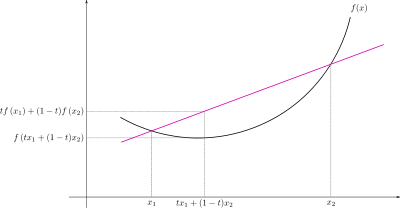
\includegraphics[scale=1.0] {images/jensens.png}}
\caption{Jensen's Inequality (image courtesy Wikipedia)}
\label{fig:jensens}
\end{figure}






\bigskip
\noindent
Now, suppose we have a vector of latent variables $z$ which has probability density function (pdf) $p(z$), and that we we can \emph{easily} sample $z$ from $p(z)$. Suppose further that we have a family of functions $f(z;\theta)$ where $\theta$ is parameter vector.  Then our goal is to optimize $\theta$ such that $f(z;\theta)$ produces samples that look like $X$ with high probability (for every $X \in \mathcal{X}$) when $z$ is sampled from $p(z)$. Stated more formally, we wish to maximize the probability of each $X$ in the training set under the \emph{generative process} described by (switching notation a bit)

\begin{flalign}
p(x) = \int_{z} p(\mathbf{x}|\mathbf{z};\theta) \; p(\mathbf{z}) \; dz = \int_{z} p_{\theta}(\mathbf{x}|\mathbf{z}) \; p(\mathbf{z}) \;  dz
\label{eqn:generative}
\end{flalign}


\section{Variational Autoencoders}
Variational autoencoders attempt to approximately optimize Equation \ref{eqn:generative}.\footnote{Note that VAEs are called autoencoders because the final training objective that derives from this setup does have an encoder and a decoder, and resembles a traditional autoencoder.}
\noindent
Now, to optimize Equation \ref{eqn:generative} there are two problems which the VAE must solve. First, the VAE must describe how to define the latent variables $z$ (that is, decide what information they represent). Second, the VAE must somehow deal with the integral over $z$ (again in Equation \ref{eqn:generative}).

\subsection{Choosing the Latent Variables $z$}
\noindent
When choosing $z$, we would like to avoid manually deciding what information each dimension of $z$ encodes. We also want to avoid explicitly describing the dependencies (i.e., the structure of $\mathcal{Z}$) between the dimensions of $z$. VAEs take an novel approach to dealing with this problem: they assume that there is no simple interpretation of the dimensions of $z$, and instead assert that samples of $z$ can be drawn from a simple distribution, typically 
$\mathcal{N}(0, I)$ (here again $I$ is the identity matrix). Seems well, impossible.

\begin{figure}
\center{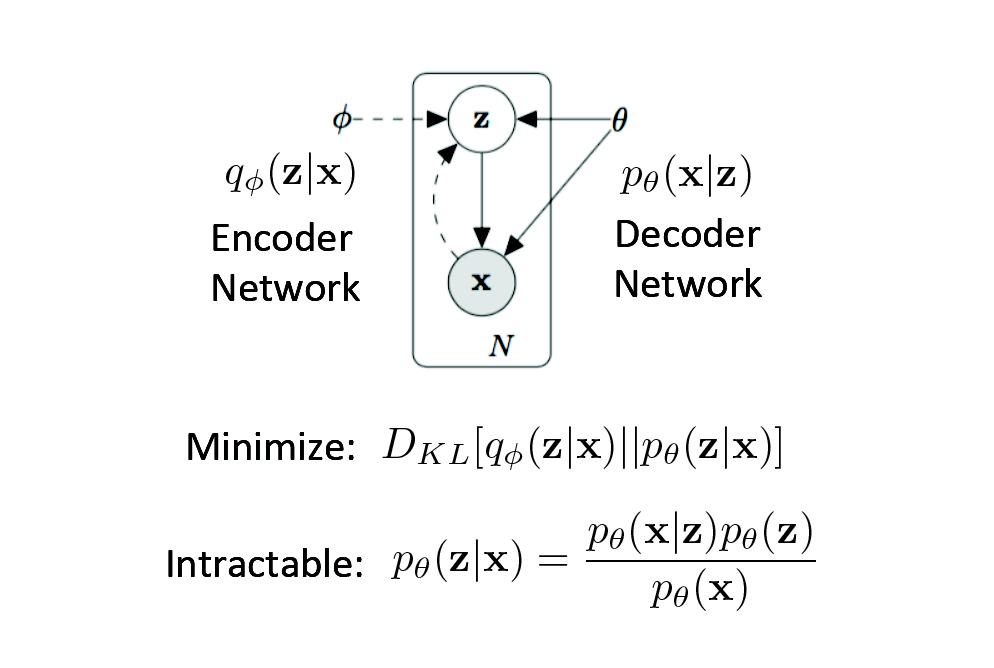
\includegraphics [scale=0.36] {images/vaedgm.png}}
\caption{The standard VAE (directed) graphical model}
\label{fig:vaegm}
\end{figure}

\bigskip
\noindent
Note that here $f(z;\theta)$ has been replaced by $p_{\theta}(\mathbf{x}|\mathbf{z})$ to make the dependence on $\mathbf{x}$ explicit. In VAEs the 
choice of $p_{\theta}(\mathbf{x}|\mathbf{z})$ is oftten a Gaussian such that 

\bigskip
\begin{flalign}
p_{\theta}(\mathbf{x}|\mathbf{z})= \mathcal{N}(f(\mathbf{z};\theta), \sigma^{2} * I)
\label{eqn:gaussian}
\end{flalign}

\bigskip
\noindent
That is, $p_{\theta}(\mathbf{x}|\mathbf{z})$ is a Gaussian distribution with mean $\mu = f(z;\theta)$ and covariance $\Sigma = \sigma^2 * I$, where $\sigma$ is a scalar hyper-parameter and $I$ is the identity matrix. The important property here is that $p_{\theta}(\mathbf{x}|\mathbf{z})$  can be efficiently computed. 


\bigskip
\noindent
So what is really going on here? The key is to notice that any distribution in $d$ dimensions can be generated by taking a set of $d$ variables that are normally distributed and mapping them through a sufficiently complicated function. Hence, provided powerful function approximators, we can simply learn a function which maps our independent, normally-distributed $\mathbf{z}$ values to whatever latent variables might be needed for the model, and then map those latent variables to $\mathbf{x}$. In fact, recall that $p_{\theta}(\mathbf{x}|\mathbf{z}) = \mathcal{N}(f (\mathbf{z}; \theta), \sigma^2 * I)$. Now, imagine that  $f (z; \theta)$ is a multi-layer neural network, then we can imagine the network using its first few layers to map the normally distributed $z$'s to the latent values with exactly the right properties.  So in the case of something like MNIST, it can use later layers to map those latent values to a fully-rendered digit. In general, we don't need to worry about ensuring that the latent structure exists. If such latent structure helps the model accurately reproduce (i.e. maximize the likelihood of) the training set, then the network will learn that structure at some layer.

\bigskip
\noindent
Recall that our goal is to maximize Equation \ref{eqn:generative} where $p(\mathbf{z}) = \mathcal{N}(0,I)$. 
Note that it is actually conceptually straightforward to compute an approximation of $p(\mathbf{x})$. To do this, in theory we can first sample a large number of $z$ values $\{z_1, \cdots, z_n\}$, and then compute 
$p(\mathbf{x}) = \frac{1}{n} \sum\limits_{i = 1}^{n} p(\mathbf{x}|z_i)$. The problem is that if $\mathcal{Z}$ is a high-dimensional space, $n$ may need to be impractically large to get an accurate estimate of $p(\mathbf{x})$; see Appendix \ref{sec:ergodic} on the Ergodic Theorem.

\section{VAE Objective Function}

So OK, the naive approach requires too many samples from $\mathcal{Z}$ to be practical. However, what we can observe is that for most of the $\mathbf{z}$'s, $p_{\theta}(\mathbf{x}|\mathbf{z})$ will be close to zero and thus add little to our estimate of $p_{\theta}(\mathbf{x})$. This leads us to one of the key ideas behind VAEs: VAEs attempt to sample values of $\mathbf{z}$ that are likely to have produced $\mathbf{x}$, and then uses those $\mathbf{z}$'s to compute $p_{\theta}(\mathbf{x})$.

\subsection{So where do the $\mathbf{z}$'s come from?}

\bigskip
\noindent
The problem with directly computing the $\mathbf{z}$'s is that posterior $p(\mathbf{z} | \mathbf{x})$ is intractable, but we need it to train the directed model. This situation is depicted in Figure \ref{fig:vae_directed}. The solution taken by VAEs is introduce an inference machine 
$q_{\phi}(\mathbf{z} | \mathbf{x})$ that \emph{learns} to approximate the posterior 
$p_{\theta}(\mathbf{z} | \mathbf{x})$. But how?


\begin{figure}
\center{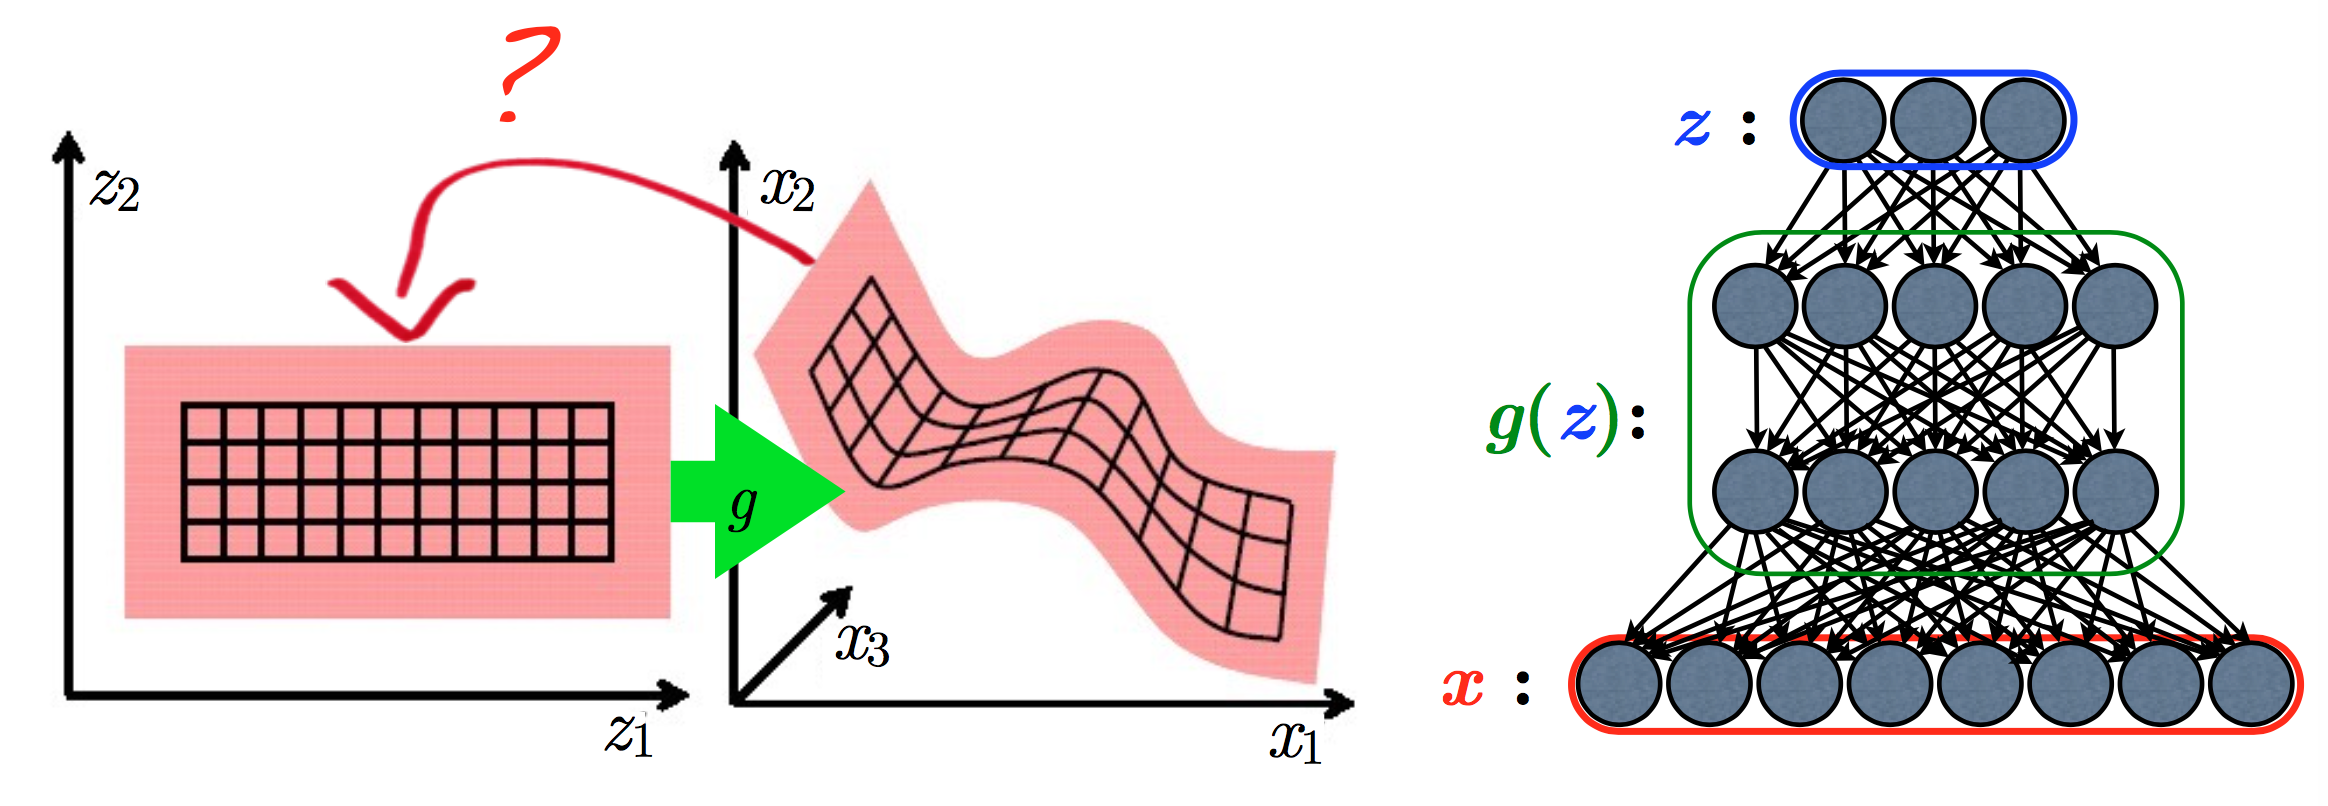
\includegraphics [scale=0.35] {images/training_directed_model.png}}
\caption{The VAE (directed) Inference/Learning Challenge. Image courtesy \url{http://videolectures.net/deeplearning2015_courville_autoencoder_extension/}}
\label{fig:vae_directed}
\end{figure}

\bigskip
\noindent
Suppose that $\mathbf{z}$ is sampled from some arbitrary distribution with pdf $q_{\phi}(\mathbf{z})$ (not the Gaussian we discussed above). This leads to one of the VAEs key operations: the relationship between 
$E_{z \sim~q_{\phi}(\mathbf{z})} [p_{\theta}(\mathbf{x}|\mathbf{z})]$ and $p(\mathbf{x})$. But how to do this? One way is to use the Kullback-Leibler divergence $\mathcal{D}_{\text{KL}}$ between $q_{\phi}(\mathbf{z})$ and $p_{\theta}(\mathbf{z}|\mathbf{x})$. That is


\begin{flalign}
\mathcal{D}_{\text{KL}}[q_{\phi}(\mathbf{z}) || p_{\theta}(\mathbf{z}|\mathbf{x})] =
E_{z \sim q_{\phi}(\mathbf{z})} [\log q_{\phi}(\mathbf{z}) - \log p_{\theta}(\mathbf{z}|\mathbf{x})]
\label{eqn:kl}
\end{flalign}

\bigskip
\noindent
Applying Bayes' Rule to Equation \ref{eqn:kl}, we get

\begin{flalign}
\mathcal{D}_{\text{KL}}[q_{\phi}(\mathbf{z}) || p_{\theta}(\mathbf{z} | \mathbf{x})]  = 
E_{z \sim q_{\phi}(\mathbf{z})}[\log q_{\phi} (\mathbf{z}) - \log p_{\theta}(\mathbf{x}|\mathbf{z}) -\log p_{\theta}(\mathbf{z})] + \log p(\mathbf{x})
\label{eqn:kl1}
\end{flalign}

\bigskip
\noindent 
Notice here that $\log p(\mathbf{x})$ can be taken out of the expectation because it doesn't depend on $\mathbf{z}$. 
Doing a little algebra gives us:

\begin{flalign}
\log p(\mathbf{x}) - \mathcal{D}_{\text{KL}}[q_{\phi}(\mathbf{z}) || p_{\theta}(\mathbf{z}|\mathbf{x})] = E_{z \sim q}[\log p_{\theta}(\mathbf{x}|\mathbf{z})] - \mathcal{D}_{\text{KL}}[q_{\phi}(\mathbf{z})||p_{\theta}(\mathbf{z})]
\label{eqn:kl2}
\end{flalign}

\bigskip
\noindent
Equation \ref{eqn:kl2} is the basis of the VAE.  The left hand side has the quantity we want to maximize: $\log p_{\theta}(\mathbf{x})$ (plus an error term that we hope is small). The right hand side is something we can optimize via stochastic gradient descent given the right choice of $q$. That is, we have solved our problem of sampling $z$ by training a distribution $q$ to predict which values of $\mathbf{z}$ are likely to produce $\mathbf{x}$ and ignoring the rest.  In particular, on left hand side we are maximizing $\log p(\mathbf{x})$ while simultaneously minimizing $\mathcal{D}_{KL} [q_{\phi}(\mathbf{z} | \mathbf{x}) || p_{\theta}(\mathbf{z}|\mathbf{x})]$. Now,
$p_{\theta}(\mathbf{z}|\mathbf{x})$ is not something we can compute analytically: it describes the values of $\mathbf{z}$ that are likely to give rise to a sample like $\mathbf{x}$ under our model in Figure \ref{fig:vaegm}. On the other hand, the second term on the left is pulling $q_{\phi}(\mathbf{z}|\mathbf{x})$ to match $p_{\theta}(\mathbf{z}|\mathbf{x})$. Assuming we use an arbitrarily high-capacity model for $q_{\phi}(\mathbf{z}|\mathbf{x})$ then $q_{\phi}(\mathbf{z}|\mathbf{x})$ will hopefully actually match $p_{\theta}(\mathbf{z}|\mathbf{x})$, in which case this KL-divergence term will be zero, and we will be directly optimizing $\log p(\mathbf{x})$\footnote{Note side effect: we have made the intractable $p_{\theta}(\mathbf{z} | \mathbf{x})$ tractable: we can just use the computable $q_{\phi}(\mathbf{z}|\mathbf{x})$ to estimate it.}.

\bigskip
\noindent
But we can go a bit further. We can define a \emph{variational lower bound} $\mathcal{L}$  on the data likelihood such that $p_{\theta}(\mathbf{x}) \geqslant \mathcal{L}(\theta, \phi, \mathbf{x})$, where

\begin{flalign}
\mathcal{L}(\theta, \phi, \mathbf{x}) &= \mathbb{E}_{q_{\phi}(z|x)} [\log p_{\theta}(x,z) - \log q_{\phi}(z|x)] \\
&= \mathbb{E}_{q_{\phi}(z|x)} [\log p_{\theta} (x|z) + \log p_{\theta}(z) - \log q_{\phi}(z|x)] \\
& = - D_{\text{KL}}[q_{\phi}(z|x) || p_{\theta}(z)] + \mathbb{E}_{q_{\phi}(z|x)} [\log p_{\theta} (x|z)]
\end{flalign}

\bigskip
\noindent
Notes:
\begin{itemize}
\item $- D_{\text{KL}}[q_{\phi}(z|x) || p_{\theta}(z)]$ is a \emph{regularization} term
\item $\mathbb{E}_{q_{\phi}(z|x)} [\log p_{\theta} (x|z)]$ is a \emph{reconstruction} term
\item{$\mathbf{x}$ is fixed}
\item{$q_{\phi}$  can be any distribution}
\item{Since we're interested in inferring $p(\mathbf{x})$ it makes sense to construct $q$ using $\mathbf{x}$}
\item {Goal: Find $q_{\phi}(\mathbf{z}|\mathbf{x}))$ so that $\mathcal{D}_{KL} [q_{\phi}(\mathbf{z} | \mathbf{x})||p_{\theta}(\mathbf{z})]$ is close to zero}
\item{Read $p_{\theta}(\mathbf{z}| \mathbf{x})$ as "the distribution over the $\mathbf{z}$'s that could have been produced by a sample like $\mathbf{x}$ under the model in Figure \ref{fig:vaegm}", which is hopefully a smaller set than all of $p(\mathbf{z})$}.
\end{itemize}

\section{VAE Inference Model}

The approach taken by VAE's  is to introduce an inference model $q_{\phi}(z|x)$ that learns to approximate the intractable posterior $p_{\theta} (z|x)$ by optimizing the variational lower bound described above:

\begin{flalign}
\mathcal{L}(\theta, \phi, \mathbf{x}) = - D_{\text{KL}}[q_{\phi}(z|x) || p_{\theta}(z)] + \mathbb{E}_{q_{\phi}(z|x)} [\log p_{\theta} (x|z)]
\label{eqn:vae_objective}
\end{flalign}

\bigskip
\noindent
To compute $q_{\phi}(z|x)$, we parameterize another neural network as shown in Figure \ref{fig:vae_parameter}.


\begin{figure}
\center{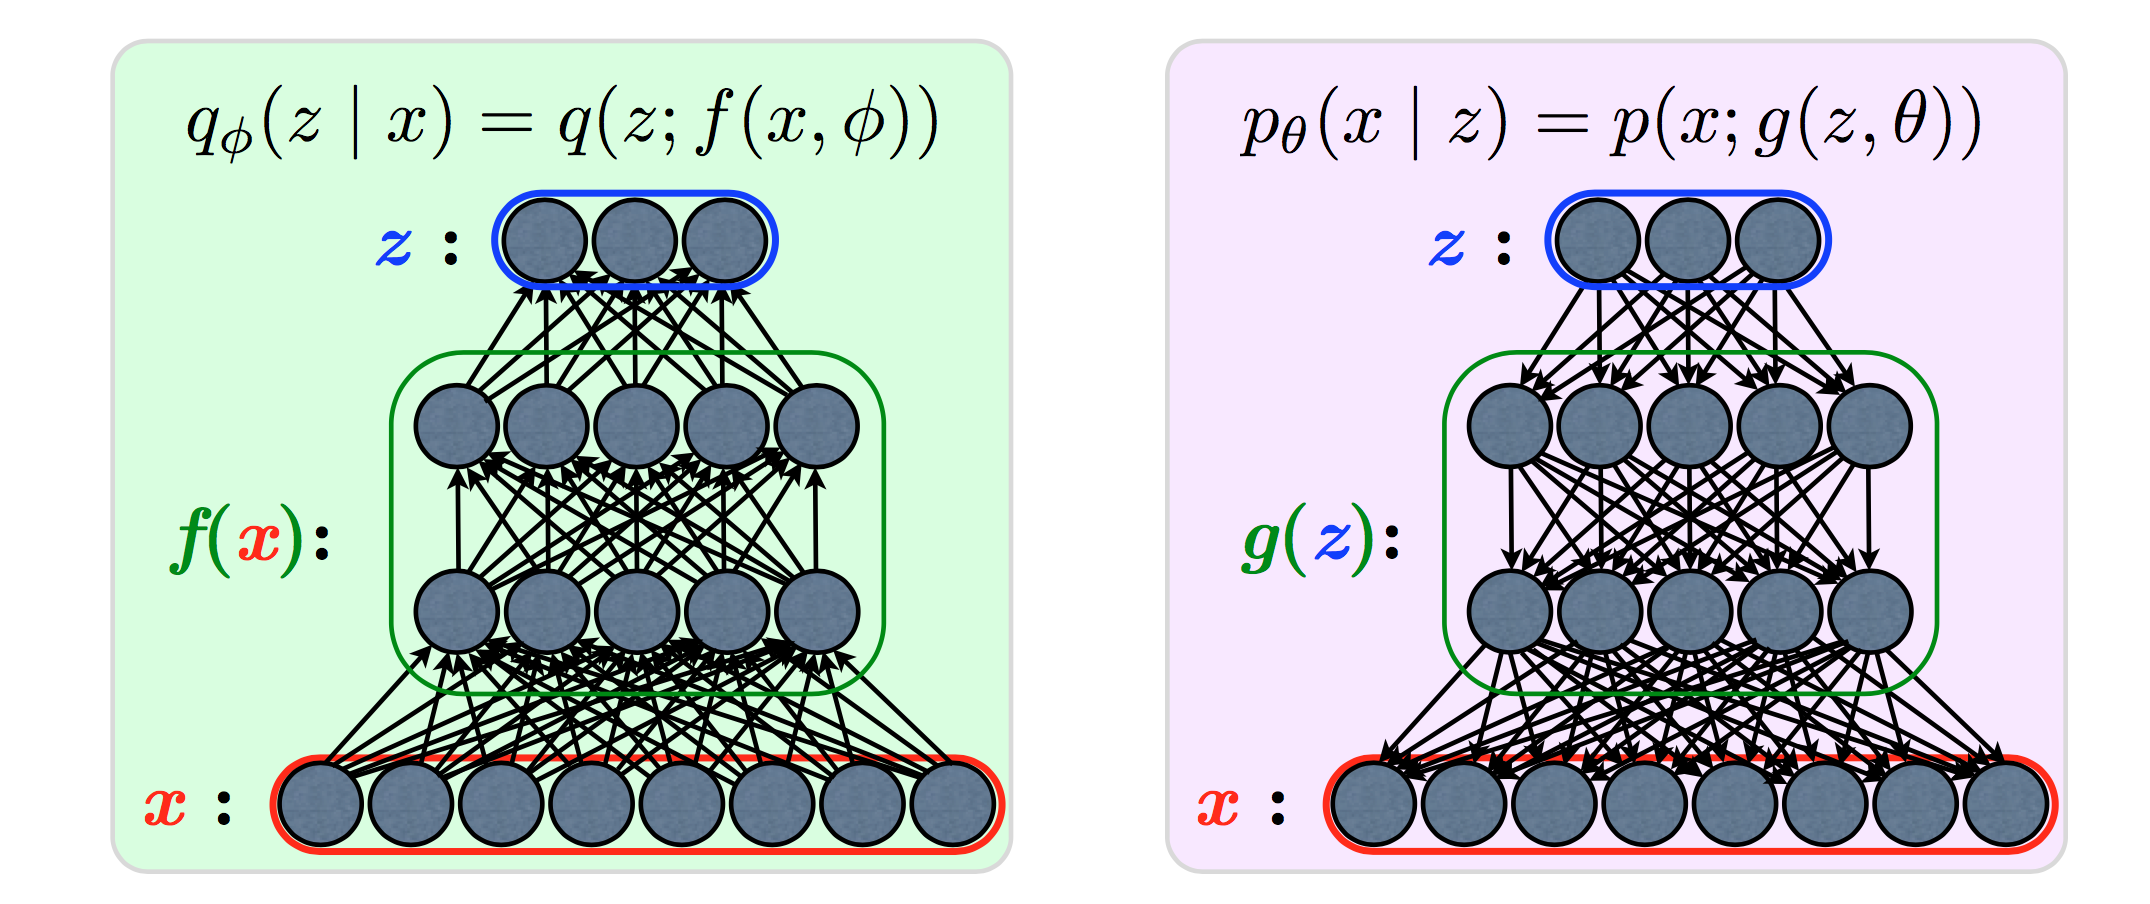
\includegraphics [scale=0.35] {images/parameterization.png}}
\caption{Neural networks for $q_{\phi}(z|x)$ and $p_{\theta}(x|z)$}
\label{fig:vae_parameter}
\end{figure}

\begin{figure}
\center{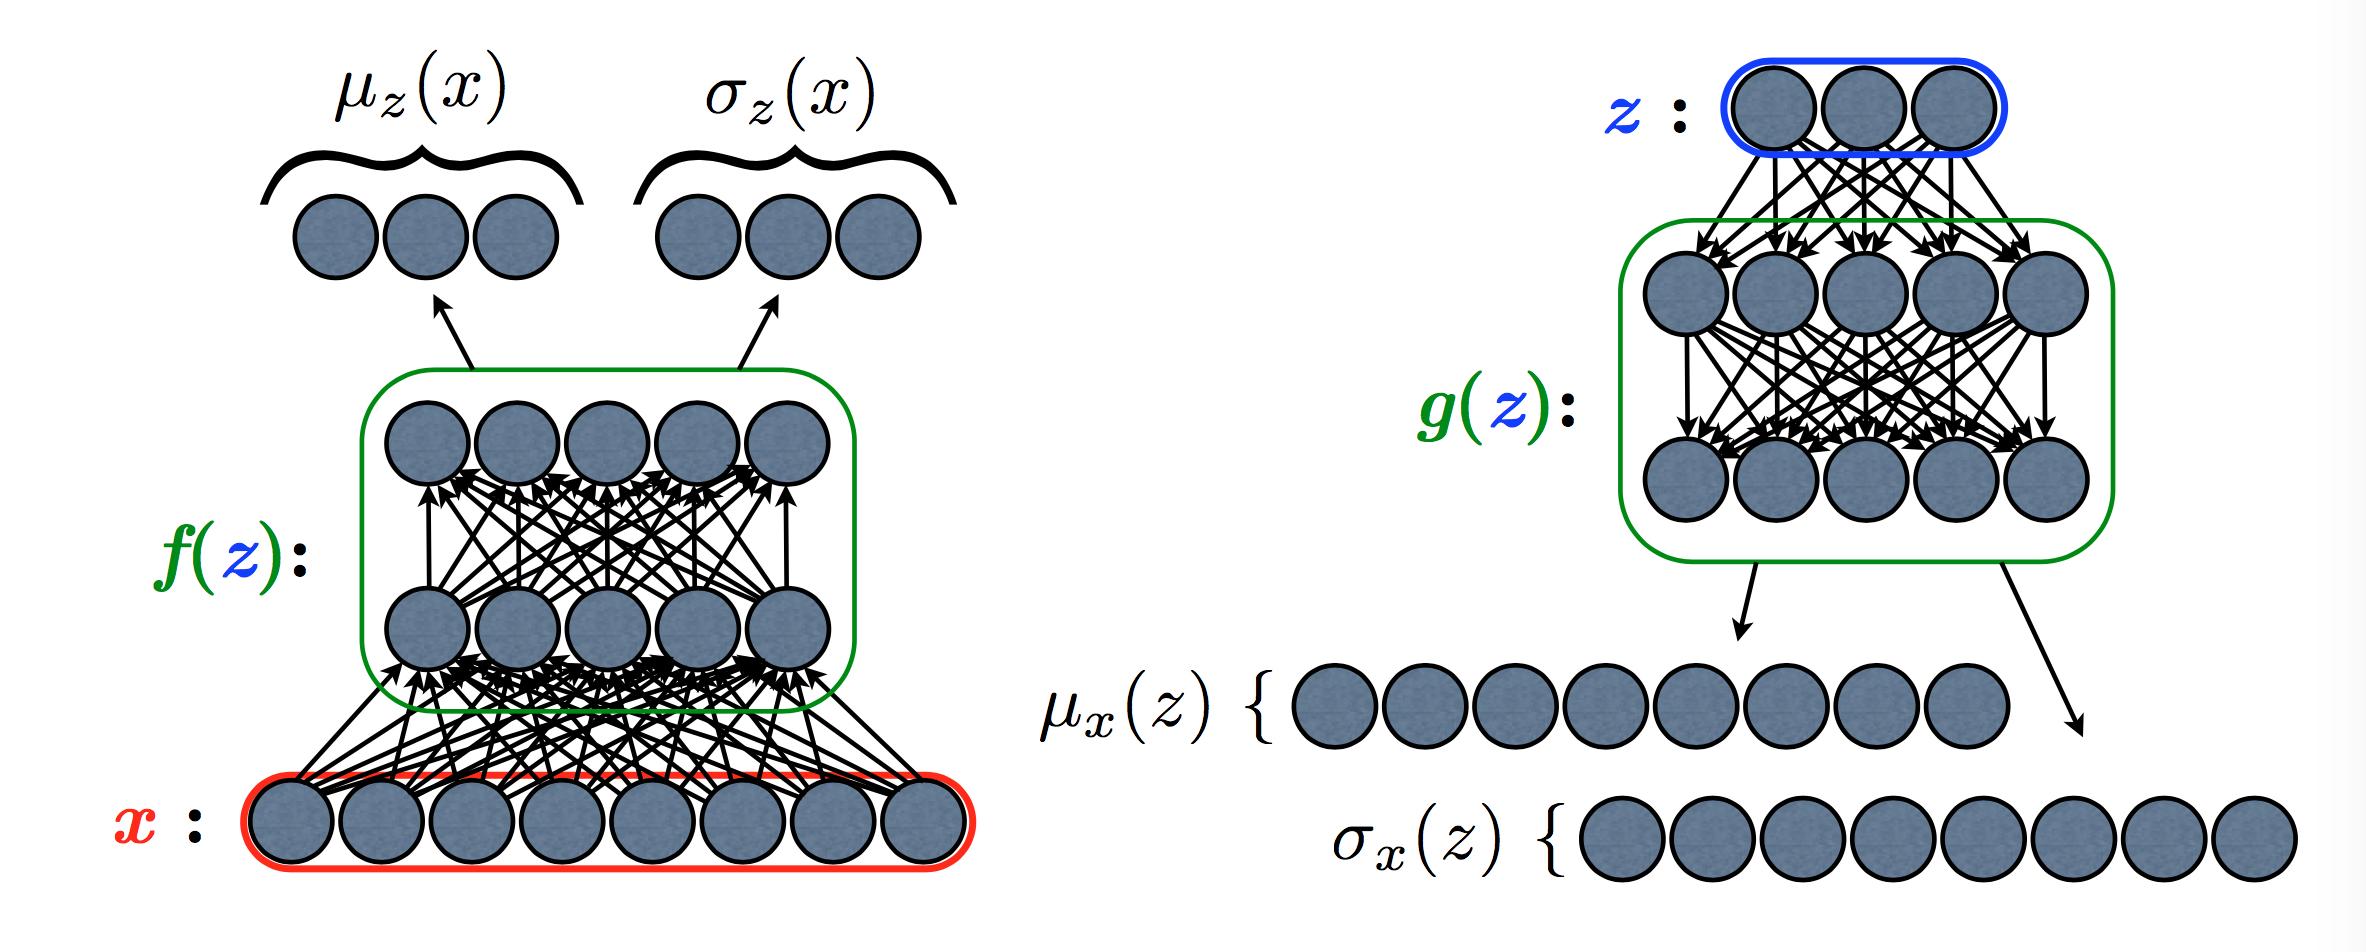
\includegraphics [scale=0.35] {images/reparam_trick.png}}
\caption{Reparameterization Trick}
\label{fig:vae_reparam_trick}
\end{figure}

\begin{figure}
\center{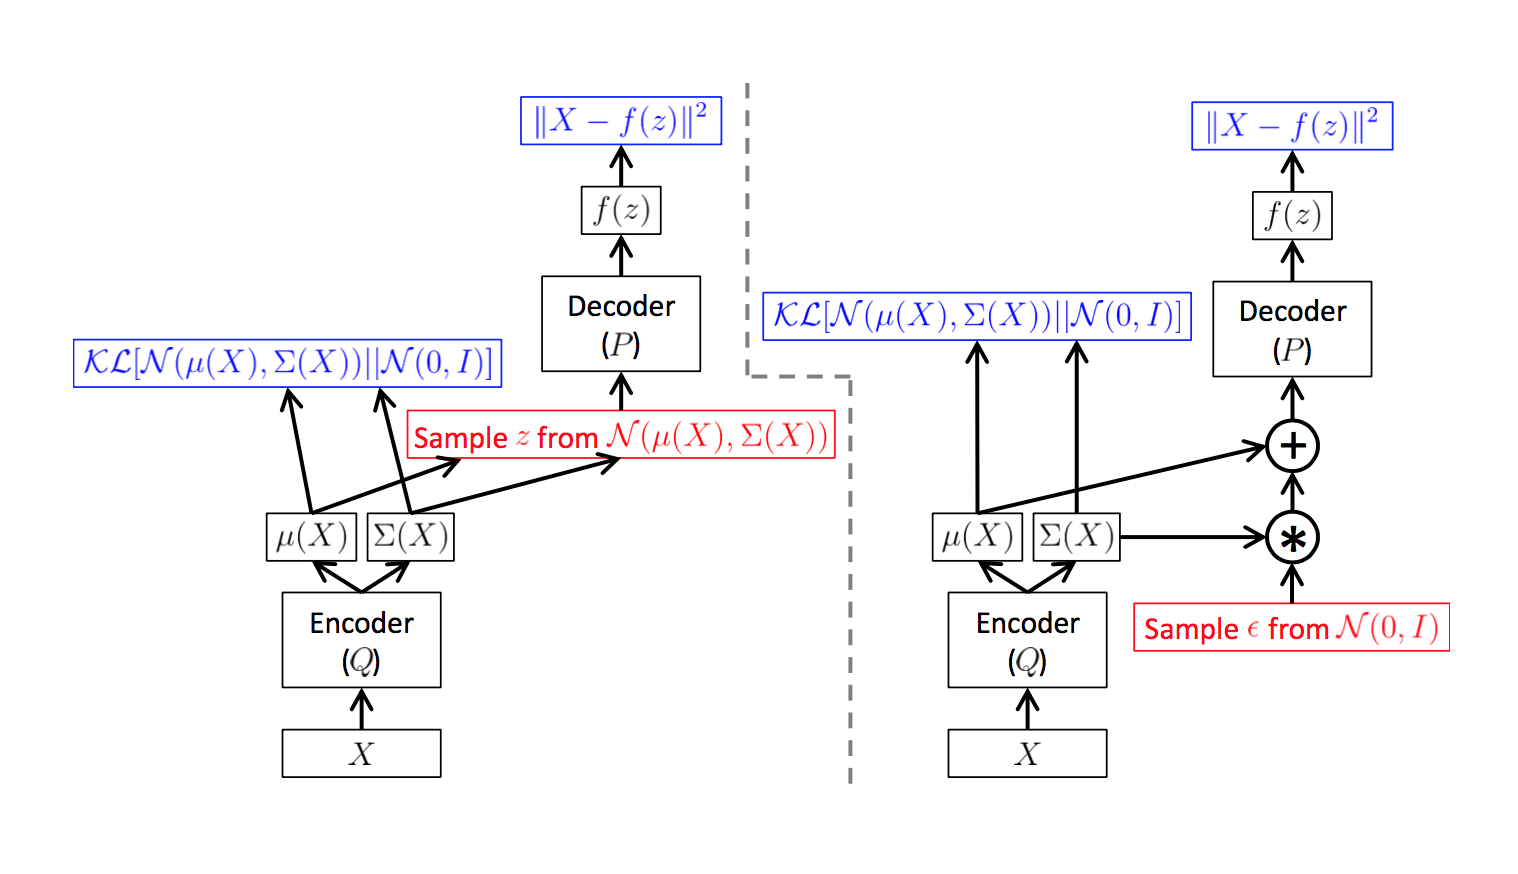
\includegraphics [scale=0.6] {images/training_time_vae.png}}
\caption{A training-time variational autoencoder implemented as a feed-forward neural network, where $p_{\theta}(\mathbf{x}|\mathbf{z})$ is Gaussian. The network on the left is without the \emph{reparameterization trick}, and network on the right is with it. Red shows sampling operations that are non-differentiable. Blue shows loss layers. The feedforward behavior of these networks is identical, but back propagation can be applied only to the right network. Image courtesy \url{https://arxiv.org/abs/1606.05908}}
\label{fig:training_time_vae}
\end{figure}

\begin{figure}
\center{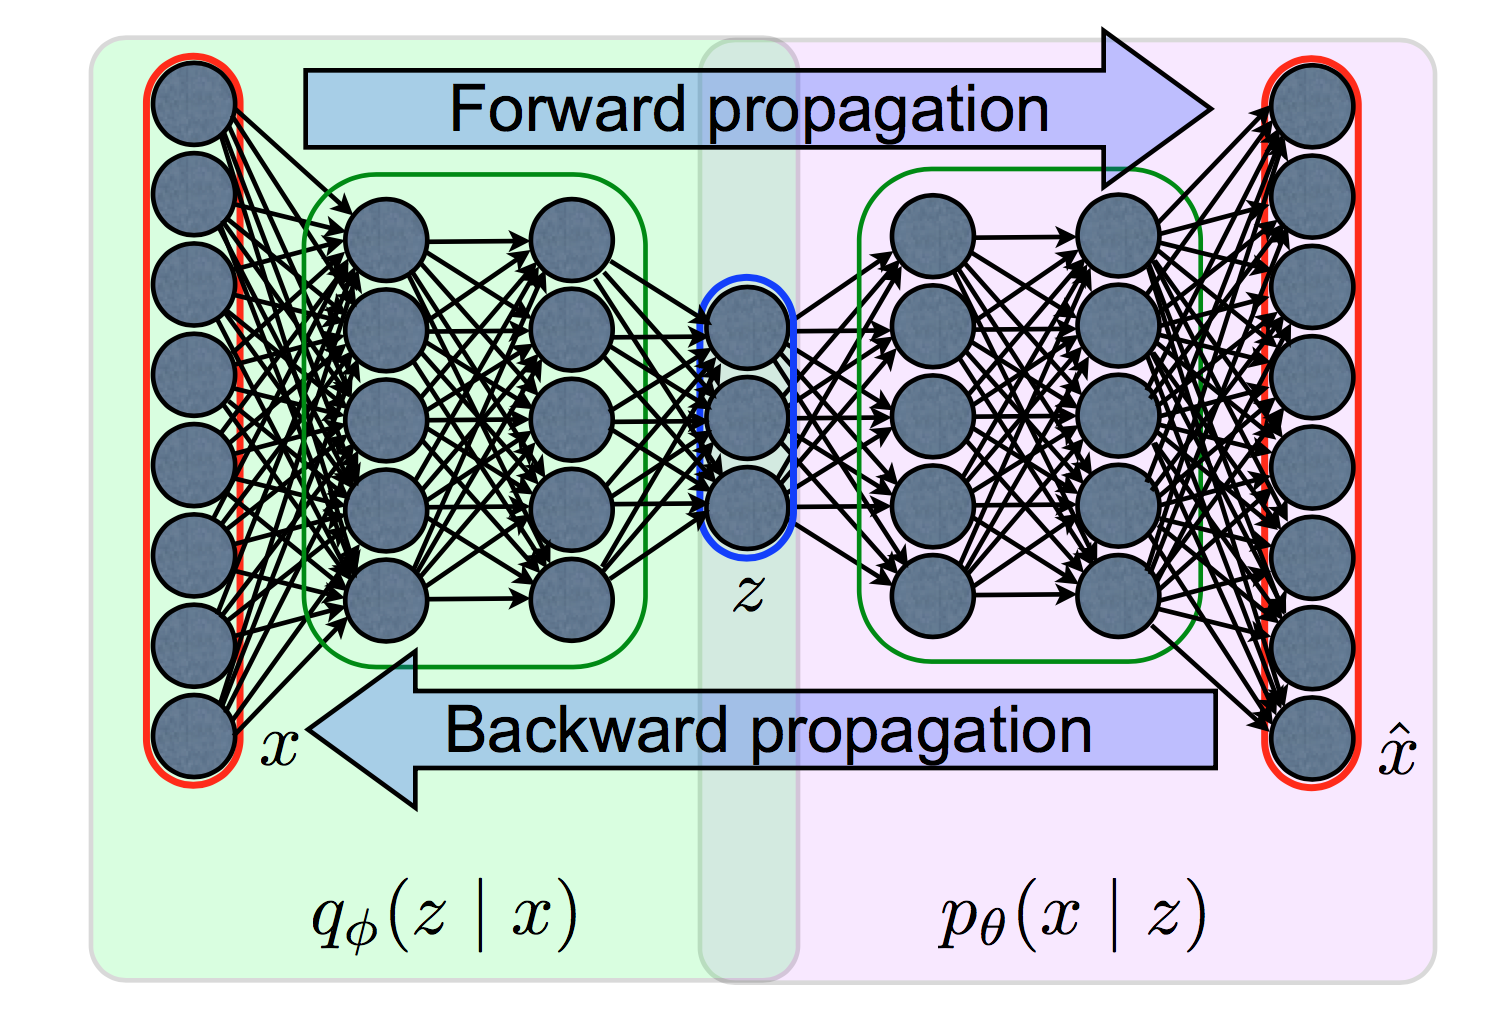
\includegraphics [scale=0.40] {images/vae_training.png}}
\caption{Training the VAE via Backpropagation}
\label{fig:vae_training}
\end{figure}

\section{One Important "Trick"}

First, consider $z$ to be real and $q_{\phi}(z|x) = \mathcal{N}(z; \mu_{z}(x), \sigma_{z}(x))$. Then the \emph{Reparameterization Trick} says we should parametrize $z$ as 
$z = \mu_{z}(x) + \sigma_{z}(x))\epsilon_{z}$, where $\epsilon_{z} = \mathcal{N}(0,1)$. This is depicted in Figure \ref{fig:vae_reparam_trick}. The beautiful thing about the reparameterization trick is that allows us to use back-propagation, moving the sampling out of the graph into the input layer at training time: see Figure \ref{fig:training_time_vae}. Note that it also to train both the encoder and decoder pathways simultaneously with the objective function shown in Equation \ref{eqn:vae_objective}. This is depicted in Figure \ref{fig:vae_training}.

\section{A Few Final Thoughts}

First, observe that once the VAE is trained, there is no need for the encoder pathway and amazingly, the VAE can generate images (in this case) directly from $\mathcal{N}(0,I)$, as incredible as that may sound. This why the VAE graphical model is frequently drawn as seen in Figure \ref{fig:vae_no_encoder}.

\begin{figure}
\center{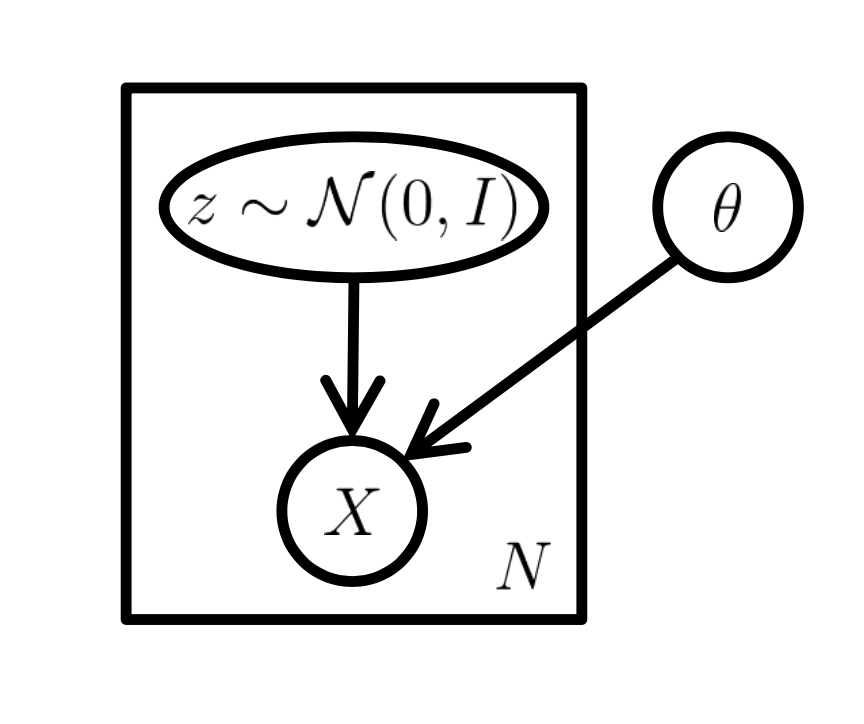
\includegraphics [scale=0.50] {images/vae_no_encoder.png}}
\caption{VAE Graphical Model With No Encoder Pathway}
\label{fig:vae_no_encoder}
\end{figure}

\bigskip
\noindent
Finally, Figure \ref{fig:vae_cost} shows an implementation of the VAE cost function from \cite{Kingma:2013aa}.


\section{Acknowledgements}

% \newpage
\bibliographystyle{plain}
\bibliography{/Users/dmm/papers/bib/vae.bib}

\section{Appendix}
\subsection{Strong Law of Large Numbers}
\label{sec:slln}

Let $X_{1}, X_{2}, \hdots, X_{M}$ be a sequence of \textbf{independent} and \textbf{identically distributed} random variables, each having a finite mean $\mu_i = E[X_{i}]$. 

\bigskip
\noindent
Then with probability 1
\begin{equation}
\frac{1}{M}\sum\limits_{i=1}^{M} X_i \rightarrow E[X]
\end{equation}
as  $M \rightarrow \infty$.

\subsection{Ergodic Theorem}
\label{sec:ergodic}
Let $\theta^{(1)}, \theta^{(2)}, \hdots, \theta^{(M)}$ be $M$ samples from a Markov chain that is \emph{aperiodic}, \emph{irreducible}, and \emph{positive recurrent}\footnote{In this case, the chain is said to be \emph{ergodic}.}, and $E[g(\theta)] < \infty$.

\bigskip
\noindent
Then with probability 1
\begin{equation}
\frac{1}{M}\sum\limits_{i = 1}^{M} g(\theta_{i}) \rightarrow E[g(\theta)]  = \int_{\Theta}^{}g(\theta) \: \pi(\theta) \:d\theta
\end{equation}
as $M \rightarrow \infty$ and where $\pi$ is the stationary distribution of the Markov chain.


\begin{figure}
\center{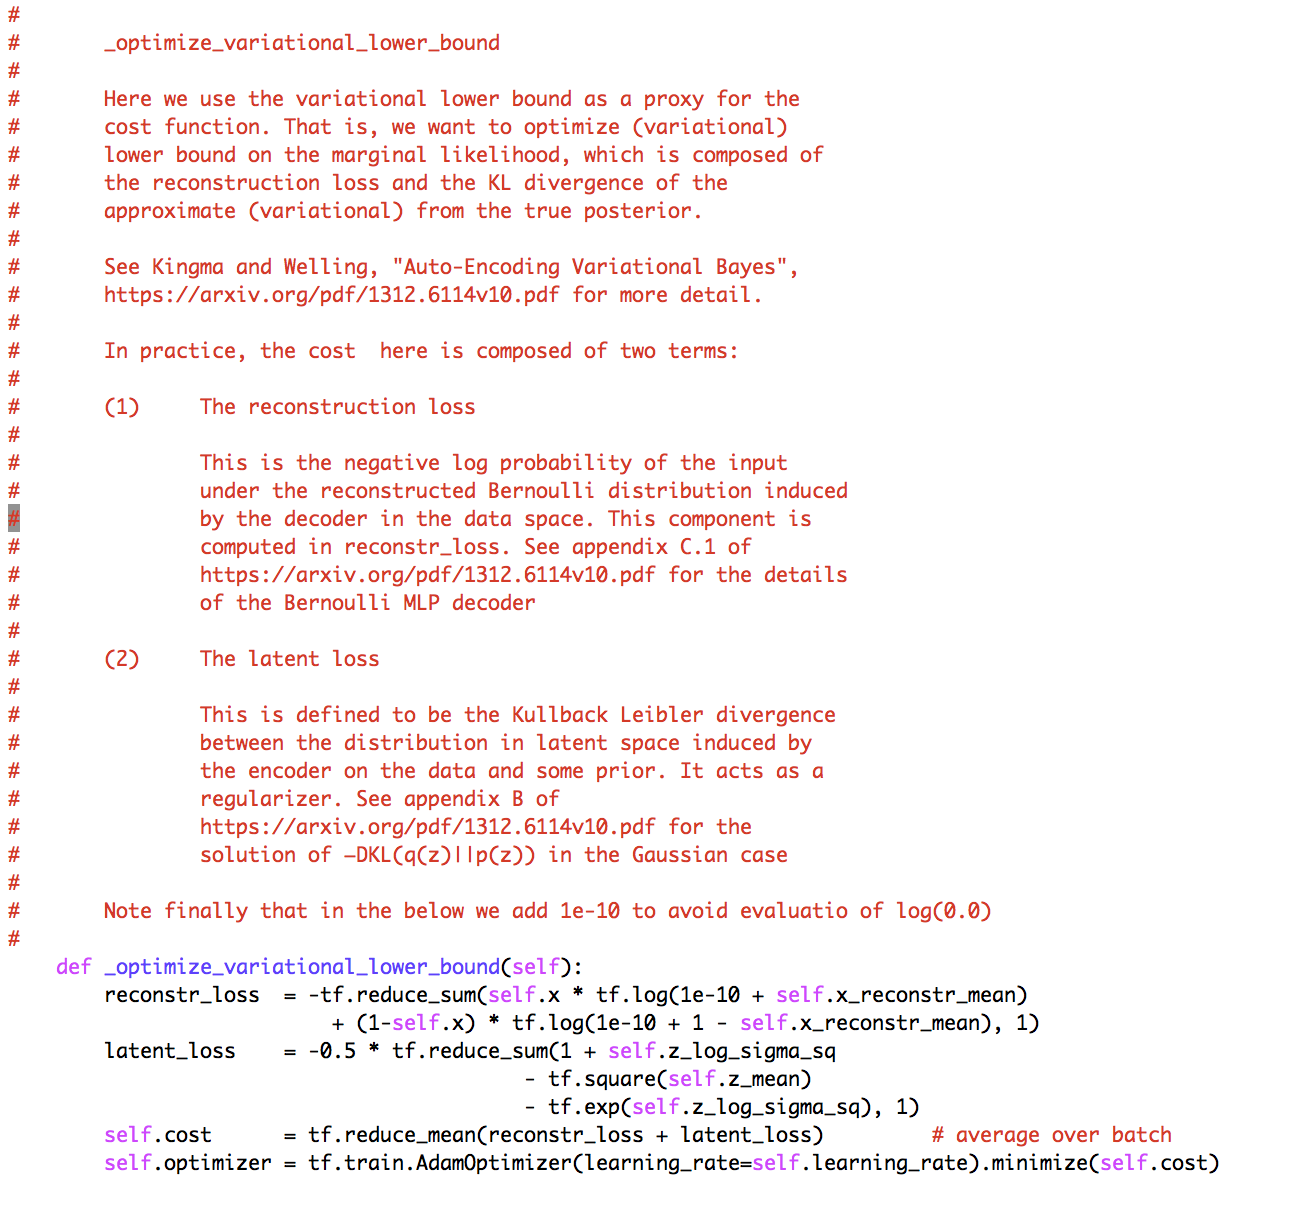
\includegraphics [scale=0.75] {images/cost.png}}
\caption{Cost Function from "Auto-encoding Variational Bayes"}
\label{fig:vae_cost}
\end{figure}



\end{document} 

